%
% File acl2015.tex
%
% Contact: car@ir.hit.edu.cn, gdzhou@suda.edu.cn
%%
%% Based on the style files for ACL-2014, which were, in turn,
%% Based on the style files for ACL-2013, which were, in turn,
%% Based on the style files for ACL-2012, which were, in turn,
%% based on the style files for ACL-2011, which were, in turn, 
%% based on the style files for ACL-2010, which were, in turn, 
%% based on the style files for ACL-IJCNLP-2009, which were, in turn,
%% based on the style files for EACL-2009 and IJCNLP-2008...

%% Based on the style files for EACL 2006 by 
%%e.agirre@ehu.es or Sergi.Balari@uab.es
%% and that of ACL 08 by Joakim Nivre and Noah Smith

\documentclass[11pt]{article}
\usepackage[english]{babel}
\usepackage{acl2015}
\usepackage{url}
\usepackage{latexsym}
\usepackage{graphicx}
\usepackage{subcaption}
\usepackage[english]{babel}
\usepackage{fancyhdr}

\pagestyle{fancy}
\fancyhf{}
\fancyhead[RE,LO]{}
\fancyhead[RE,LO]{}
\fancyfoot[CE,CO]{CS230 Stanford University Project Milestone}
\fancyfoot[LE,RO]{\thepage}
\renewcommand{\headrulewidth}{0pt} 

\setlength\titlebox{3cm}

% You can expand the titlebox if you need extra space
% to show all the authors. Please do not make the titlebox
% smaller than 5cm (the original size); we will check this
% in the camera-ready version and ask you to change it back.


\title{Learning to Play Minichess Without Human Knowledge}

\author{
  { Karthik selvakumar Bhuvaneswaran} \\
  {\tt karthik0@stanford.edu}
}

\date{May 19th 2018}

\usepackage{listings}
\usepackage{color}

\definecolor{dkgreen}{rgb}{0,0.6,0}
\definecolor{gray}{rgb}{0.5,0.5,0.5}
\definecolor{mauve}{rgb}{0.58,0,0.82}
\lstset{frame=tb,
  language=Python,
  aboveskip=3mm,
  belowskip=3mm,
  showstringspaces=false,
  columns=flexible,
  basicstyle={\small\ttfamily},
  numbers=none,
  numberstyle=\tiny\color{gray},
  keywordstyle=\color{blue},
  commentstyle=\color{dkgreen},
  stringstyle=\color{mauve},
  breaklines=true,
  breakatwhitespace=true,
  tabsize=3
}

\begin{document}
\maketitle
\begin{abstract}

Implementing a self play based algorithm using neural networks has become popular after the tremendous success of Alpha Zero by Deep Mind in the game of go. Replicating the results for a game with smaller search space like TicTacToe, Connect4 etc has already been proven in alpha-zero-general \cite{alphazerogeneral}, but for games with larger search space like chess requires scaling.
In this paper we apply scaled up version of alpha-zero-general for the game of Minichess and evaluate our learning algorithm with random and greedy baselines. 

\end{abstract}


\section{Introduction}

It was estimated that games like Go, which have a large branching factor, and where it is very difficult to determine the likely winner from a non-terminal board position, would not be solved for several decades. However, AlphaGo (Silver et al. 2016), which uses recent deep reinforcement learning and Monte Carlo Tree Search methods, managed to defeat the top human player, through extensive use of domain knowledge and training on the games played by top human players. Many of the existing approaches for designing systems to play games relied on the availability of expert domain knowledge to train the model on and evaluate non-terminal states. Recently, however, AlphaGo Zero (Silver et al. 2017b) described an approach that used absolutely no expert knowledge and was trained entirely through self-play. This new system, AlphaGo Zero, even outperforms the earlier AlphaGo model. This represents a very exciting result, that computers may be capable of superhuman performances entirely through self-learning, and without any guidance from humans. In our work, we extract ideas from the AlphaGo Zero paper and apply them to the game of Minichess. We use board sizes of 5x5, for which learning through self-play usually takes 5 to 7 days in a single CPU/GPU, but can be trained within a day with a distributed setup of multiple CPU/GPU. For evaluation, we compare our trained agents to random and greedy baselines.


\section{Related Work}

DeepMind published a ​paper​ of Alpha Zero on arXiv that extends AlphaGo Zero methods to Chess and Shogi. However, the code is not open source and will not be released by DeepMind. Moreover, they use about 5000 TPUs to generate games in parallel. This makes it very difficult to replicate the results and extend the work to other games. ​Alpha Zero General​ is open source single-thread single-GPU version that works for any game and any framework (currently PyTorch, TensorFlow and Keras). It works quite well on small games such as 6x6 Othello after ​2-3 days of training on a single GPU​. We will be extending Alpha Zero General project by analyzing the components that can be parallelized and training a Neural Network for the game of Minichess. 


\section{Methods}

We provide a high-level overview of the algorithm we employ, which is based on the AlphaGo Zero (Silver et al. 2017b) paper. The algorithm is based on pure self-play and does not use any human knowledge except knowing the rules of the game. At the core, we use a neural network that evaluates the value of a given board state and estimates the optimal policy. The self-play is guided by a Monte-Carlo Tree Search (MCTS) that acts as a policy improvement operator. The outcomes of each game of self-play are then used as rewards, which are used to train the neural network along with the improved policy. Hence, the training is performed in an iterative fashion- the current neural network is used to execute self-play games, the outcomes of which are then used to retrain the neural network. The following sections describe the different components of our system in more detail. 

\subsection{Gameplay}

A 5x5 board is the smallest board on which one can set up all kind of chess pieces as a start position. We consider Gardner's minichess variant in which all pieces are set as in a standard chessboard (from Rook to King). This game has roughly $9 * 10^{18}$ legal positions \cite{gardner} and is comparable in this respect with checkers.


\begin{figure}[h!]
  \centering
  \begin{subfigure}[b]{0.3\linewidth}
    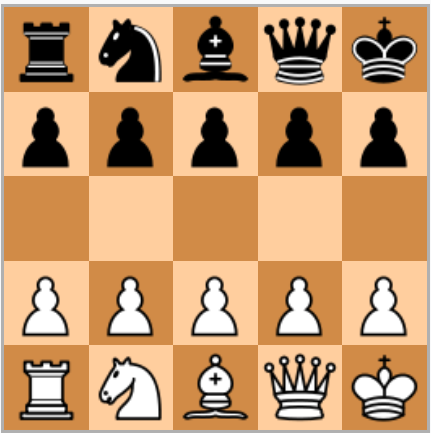
\includegraphics[width=\linewidth]{gardner.png}
  \end{subfigure}
  \caption{Gardner Minichess layout (5X5)}
  \label{fig:gameplay}
\end{figure}

\subsection{Neural Network Architecture}

We use a neural network parameterized by $\theta$ that takes as input the board state $s$ and outputs the continuous value of the board state $v_{\theta}$ $\epsilon$ [-1,1] from the perspective of the current player, and a probability vector $\vec{p}$ over all possible actions. $\vec{p_{\theta}}$ represents a stochastic policy that is used to guide the self-play. The neural network is initialized randomly. At the end of each iteration of self-play, the neural network is provided training examples of the form ($s_{t}$,$\vec{\pi_{t}}$,$z_{t}$). $\vec{\pi_{t}}$ gives an improved estimate of the policy after performing MCTS starting from st, and $z_{t}$ $\epsilon$ [-1,1] is the final outcome of the game from the perspective of the current player. The neural network is then trained to minimize the following loss function:

\[ l = \sum (v_{\theta}(s_{t}) - z_{t})^{2}+ \vec{\pi_{t}} log(\vec{p_{\theta}}(s_{t}))  \]

\begin{figure}[h!]
  \centering
  \begin{subfigure}[b]{1\linewidth}
    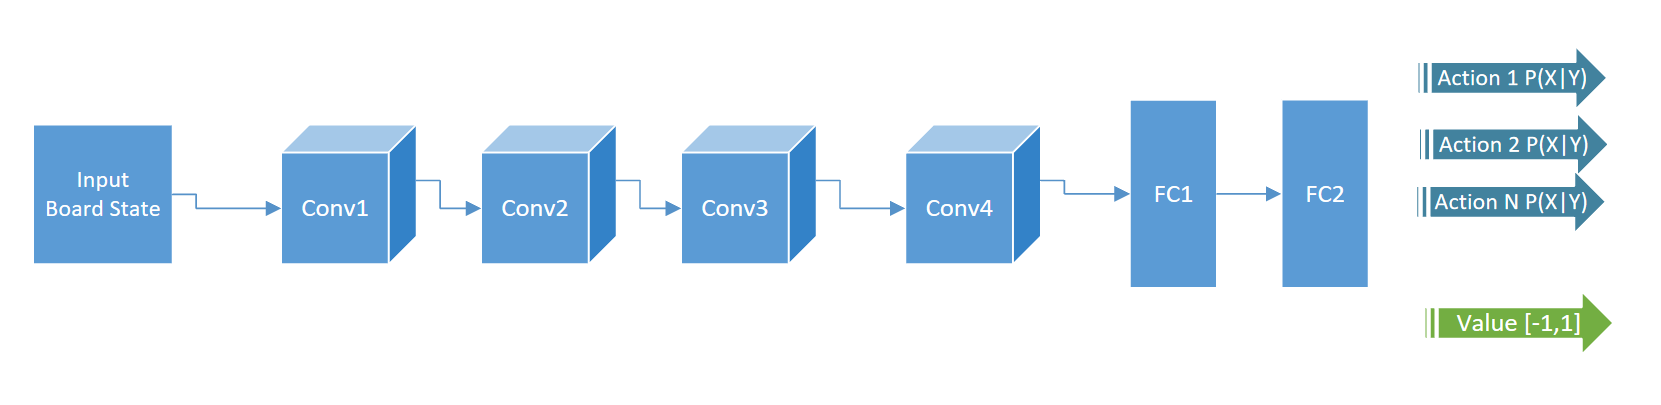
\includegraphics[width=\linewidth]{cnn.png}
  \end{subfigure}
  \caption{Neural Network Architecture}
  \label{fig:gameplay}
\end{figure}
 
  We use a neural network that takes the raw board state as the input. This is followed by 4 convolutional networks and 2 fully connected feed forward networks. This is followed by 2 connected layers - one that outputs $v_{\theta}$ and another that outputs the vector $\vec{p_{\theta}}$. Training is performed using the Adam (Kingma and Ba 2014) optimizer with a batch size of 512, with a dropout (Srivastava et al. 2014) of 0.3, and batch normalization (Ioffe and Szegedy 2015). The code is implemented in Keras backed up by tensorflow-gpu. 
  

\subsection{Distributed Architecture}

Our experiments were ran on AWS EC2 instances, but architecture is generic for all cloud services. 
Following table explains the different components and type of instance created in AWS. 

\begin{figure}[h!]
  \centering
  \begin{subfigure}[b]{1\linewidth}
    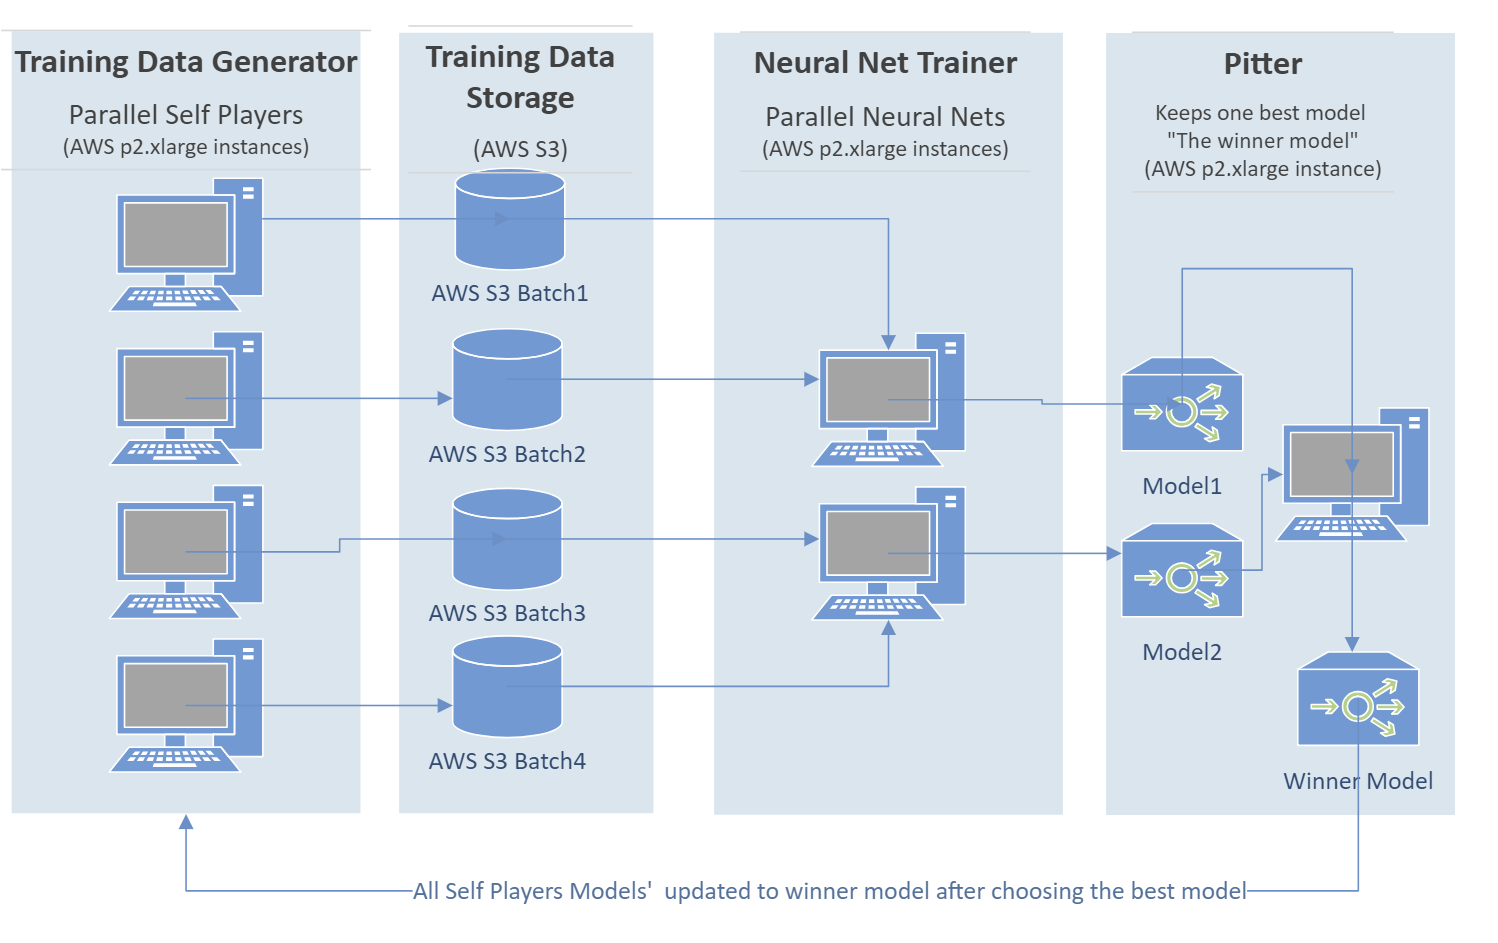
\includegraphics[width=\linewidth]{distributed_arch.png}
  \end{subfigure}
  \caption{Distributed Architecture in AWS}  
  \label{fig:distributed_arch}
\end{figure}

\begin{table}[h]
\begin{center}
\begin{tabular}{c c}
\hline \bf Component Name & \bf Instances \\ \hline
Training Data Generator & 4 x p2.xlarge \\
Training Data Storage & 1 x AWS S3 \\
Neural Net Trainer & 2 x p2.4xlarge \\
Pitter & 1 x p2.xlarge \\
\hline
\end{tabular}
\end{center}
\caption{\label{font-table} Components in Scaled Setup}
\end{table}


\subsection{Data Generation through Self Play}

{\em Training Data Generator} component is responsible for carrying out self plays and generating dataset required for training our Neural Network. It creates two players and plays the game till the ends state (Won/Lost/Draw). On every move, it collects three data points: board state, policy output and value output of the network. This dataset is then uploaded to AWS S3 which will be consumed by {\em Neural Net Trainer}. We use only one neural network to calculate both policy and value, with the help of Monte Carlo Tree Search (MCTS). At any point of time, currently known best model is used and the network becomes smarter and smarter after training for more iterations with larger training data.


\subsection{Neural Net Trainer}

{\em Neural Net Trainer} component performs the training and needs to be more powerful to crunch the enormous amount of batch data generated by self play and perform several iterations of gradient descent. Hence it is chosen to be four times powerful than {\em Training Data Generator} in terms of number of physical GPU hardware and CPU concurrency. This component performs training and outputs the model with lower loss. 

  
\subsection{Pitter and best model selection}

{\em Pitter} component takes all the models from {\em Neural Net Trainers} and performs pitting. Depending on the winner the best model is updated and all the {\em Training Data Generators} are updated with this latest model, which helps in improving the quality of Training data being generated, eventually leading to an expert model.


\section{Experiments}

We ran experiments on a 5X5 version of Chess referred as Minichess. We used 250 MCTS simulation per move which is good enough simulation for a 5X5 board. With 10 episodes per training iteration and 100 iterations of training it took 2 hours of simulation. This experiment needs to be carried out with bigger training set and larger iterations for better results. Initially system crashes with memory dump error several times, since the MCTS simulation is the bottleneck. 

Inorder to scale the training, any MCTS search beyond 1000 search deep will be considered as draw. This happened in scenarios when there is only White King and Black King left on the board and both players cannot bring the game to an end. This draw state is tailored for subset of board games like Minichess and might lead to erroneous prediction for other board games where the valid simulation might itself be more than 1000 level deep.

\subsection{Baselines}

We implemented two baselines for comparison with our trained AI Player. The first is a random player baseline. A random player chooses from one of the valid moves randomly at each step in the game. The second is a greedy player which chooses a move that causes the attack which maximizes the score. For computing score each Piece is assigned a weight. Weights are only used for Greedy player and never used for neural network training or MCTS search for the purpose of extendability of this architecture to different game.

The results of the different baselines are listed in Table.

\begin{table}[h]
\begin{center}
\begin{tabular}{c c c c}
\hline \bf Baseline & \bf CNN & \bf Resnet  & \bf Densenet   \\ \hline
Random & 14/20 & In Progress & In Progress  \\
Greedy & In Progress & In Progress & In Progress \\

\hline
\end{tabular}
\end{center}
\caption{\label{font-table} Performance on 5X5 chess layouts }
\end{table}

\section{Conclusion}
\label{sec:conclusion}

Our model performs better than Random player, but still looses reasonable number of games. Our goal is to defeat Random player in all scenarios and perform atleast 60\% better than Greedy Player. Inorder to improve the performance we are working on the following steps:

\begin{itemize}
	\item[1] Train with larger data set for longer iterations 
	\item[2] Perform the training on different architecture like ResNet and DenseNet 
	\item[3] Tune the hyper parameters like Dropout, Exploration, and different Activations
\end{itemize}

% include your own bib file like this:
%\bibliographystyle{acl}
%\bibliography{acl2015}

\section{Code}
Our code can be found at this Github repository under the branch minichess https://github.com/karthikselva/alpha-zero-general/tree/minichess.

\paragraph{Acknowledgment}

Thanks to Patrick Cho for his direction and excellent mentorship and rest of the staff for helping us understand the architecture behind the beautiful AlphaZero.


\begin{thebibliography}{}

\bibitem[\protect\citename{Mehdi Mhalla et al}2013]{gardner}
\newblock [Mehdi Mhalla, Frederic Prost 2013]
\newblock Gardner's Minichess Variant is solved. {\em arXiv e-print (arXiv:1307.7118) }

\bibitem[\protect\citename{Surag Nair et al}2017]{alphazerogeneral}
\newblock [Surag Nair, Shantanu Thakoor, Megha Jhujhunwala 2016]
\newblock Learning to Play Othello Without Human Knowledge {\em github.com/suragnair/alpha-zero-general}

\bibitem[\protect\citename{Silver et al.}2017a]{Aho:72}
\newblock [Silver et al. 2017a] Silver, D.; Hubert, T.; Schrittwieser, J.; Antonoglou, I.; Lai, M.; Guez, A.; Lanctot, M.; Sifre, L.; Kumaran, D.; Graepel, T.; Lillicrap, T.; Simonyan, K.; and Hassabis, D.
\newblock Mastering Chess and Shogi by Self-Play with a General Reinforcement Learning Algorithm. {\em ArXiv e-prints.}

\bibitem[\protect\citename{Browne et al. 2012}2012]{Aho:73}
\newblock [Browne et al. 2012] Browne, C. B.; Powley, E.; Whitehouse, D.; Lucas, S. M.; Cowling, P. I.; Rohlfshagen, P.; Tavener, S.; Perez, D.; Samothrakis, S.; and Colton, S. 2012. 
\newblock A survey of monte carlo tree search methods. {\em IEEE Transactions on Computational Intelligence and AI in games 4(1):1–43.}

\bibitem[\protect\citename{Campbell, Hoane, and hsiung Hsu 2002}]{Aho:74} 
\newblock [Campbell, Hoane, and hsiung Hsu 2002] Campbell, M.; Hoane, A.; and hsiung Hsu, F. 2002. 
\newblock {\em Deep blue. Artificial Intelligence 134(1):57 – 83.} 

\bibitem[\protect\citename{Heinz 2001}]{Aho:75} 
\newblock [Heinz 2001] Heinz, E. A. 2001. 
\newblock New Self-Play Results in Computer Chess. {\em Berlin, Heidelberg:  Springer Berlin Heidelberg. 262–276.}

\bibitem[\protect\citename{Ioffe and Szegedy 2015}]{Aho:76} 
\newblock [Ioffe and Szegedy 2015] Ioffe, S., and Szegedy, C. 2015.
\newblock Batch normalization: Accelerating deep network training by reducing internal covariate shift. {\em In International Conference on Machine Learning, 448–456.}

\bibitem[\protect\citename{Kingma and Ba 2014}]{Aho:77} 
\newblock [Kingma and Ba 2014] Kingma, D., and Ba, J. 2014.  \newblock Adam: A method for stochastic optimization. {\em arXiv preprint arXiv:1412.6980.}

\bibitem[\protect\citename{Silver et al. 2016}]{Aho:78} 
\newblock [Silver et al. 2016] Silver, D.; Huang, A.; Maddison, C. J.; Guez, A.; Sifre, L.; van den Driessche, G.; Schrittwieser, J.; Antonoglou, I.; Panneershelvam, V.; Lanctot, M.; Dieleman, S.; Grewe, D.; Nham, J.; Kalchbrenner, N.; Sutskever, I.; Lillicrap, T.; Leach, M.; Kavukcuoglu, K.; Graepel, T.; and Hassabis, D. 2016. 
\newblock Mastering the game of go with deep neural networks and tree search.  {\em Nature 529(7587):484–489. Article.}


\bibitem[\protect\citename{Srivastava et al. 2014}]{Aho:79} 

\newblock [Srivastava et al. 2014] Srivastava, N.; Hinton, G. E.; Krizhevsky, A.; Sutskever, I.; and Salakhutdinov, R. 2014. 
\newblock Dropout: a simple way to prevent neural networks from overfitting. {\em Journal of machine learning research 15(1):1929– 1958.} 

\bibitem[\protect\citename{Van Der Ree and Wiering 2013}]{Aho:80} 

\newblock [Van Der Ree and Wiering 2013] VanDerRee, M., andWiering, M. 2013.
\newblock  Reinforcement learning in the game of othello: learning against a fixed opponent and learning from selfplay. {\em In Adaptive Dynamic Programming And Reinforcement Learning (ADPRL), 2013 IEEE Symposium on, 108–115. IEEE.}


\end{thebibliography}

\begin{table}[h]
\begin{center}
\begin{tabular}{c c c}
\hline \bf Piece & \bf White Weight & \bf Black Weight \\ \hline
Pawn & 100 & -100 \\
Knight & 280 & - 280 \\
Bishop & 320 & -320 \\
Rook & 479 & -479 \\
Queen & 929 & -929 \\
King & 60000 & -6000 \\
\hline
\end{tabular}
\end{center}
\caption{\label{font-table} Weights of each Piece on Greedy Player }
\end{table}

\end{document}